\documentclass[a4paper,12pt]{article}
\usepackage[slovene]{babel}
\usepackage[utf8]{inputenc}
\usepackage[T1]{fontenc}
\usepackage{lmodern}
\usepackage{amsmath,amsfonts,amssymb}
\usepackage{graphicx}

\title{Algoritmi - 1. Domača naloga}
\author{Timen Bobnar}
\date{22.03.2025, Ljubljanja}


\begin{document}
\setlength{\parindent}{0cm}
\maketitle

\section{Časovna zahtevnost}
\subsection{1. Naloga}
Časovna zahtevnost je $O(n)$, saj imamo le eno zanko od $0$ do $n$.

\subsection{2.Naloga}
Časovna zahtevnost je $O(n*n*log(n))$, saj imamo zanko, ki gre od $0$ do $n$, ter v njej še eno zanko kjer se na vsakem koraku število korakov razpolovi(torej logaritem). Na koncu dodamo še eno zanko, saj uporabimo prejšnjo funkcijo.

\subsection{3. Naloga}
Držimo se formule $$T(n)=a*T(n/b)+f(n)$$
Opazimo, da sta $a=b=2$ iz tega sledi, da $\epsilon = 1 $ ($f(n)=1 \in O(n^{1-\epsilon})$)
Sledi, da je $T(n)=\theta(n)$               

\section{Rodovne funkcije}
\subsection{4. Naloga}
Poznamo formulo za rodovne funkcije:
$$P(x) = \sum_{i=0}^{n} c_i x^i = c_0 + c_1 x + c_2 x^2 + c_3 x^3 + \cdots + c_{13} x^{13}$$

\begin{align*}
1 cent : \quad 1+ x + x^2 + \cdots + x^{13} \\
2 centa: \quad 1+ x^2 + x^4 + x^6 + x^8 + x^{10} + x^{12} \\
5 centov: \quad 1+ x^5 + x^{10} \\
10 centov: \quad 1+x^{10}
\end{align*}


$$ A(x) = (1+x + x^2 + \cdots + x^{13}) \cdot (1+x^2 + x^4 + \cdots + x^{12}) \cdot (1+x^5 + x^10) \cdot (1+x^{10}) = \\
- \cdots + \boxed{16} x^{13} + \cdots $$


Odgovor1 = $16$

$$P(x) = (1+x + x^2 + \cdots + x^{13}) \cdot (1+x^2 + x^4 + \cdots + x^{12}) = \cdots + \boxed{7} \cdot x^{13} + \cdots$$

Odgovor2 = $7$

\subsection{5. Naloga}
$$T_n=\frac{n(n+1)}{2}$$
$$R(x) = \sum_{i=0}^{\infty} T_i x^i = \sum_{i=0}^{\infty} \frac{i(1+i)}{2} x^i  $$
100: $ \frac{100 * 101}{2} = 5050 $

\subsection{6. Naloga}
Če spišemo rodovne funkcije potenc števila $2$ na način:
$$1+x, 1+x^2, 1+x^4, \cdots 1+x^{2^k}$$
Če sedaj vse te funkcije pomnožimo med sabo dobimo $$\sum_{i=0}^{\infty} x^i $$.
Torej lahko vidimo iz vsote, ki je rodovna funkcija, da lahko sestavimo vsa naravna števila.
Enakost, da je produkt enak vsoti lahko dokazemo z indukcijo.

\section{Turingovi stroji}
\subsection{7. Naloga}
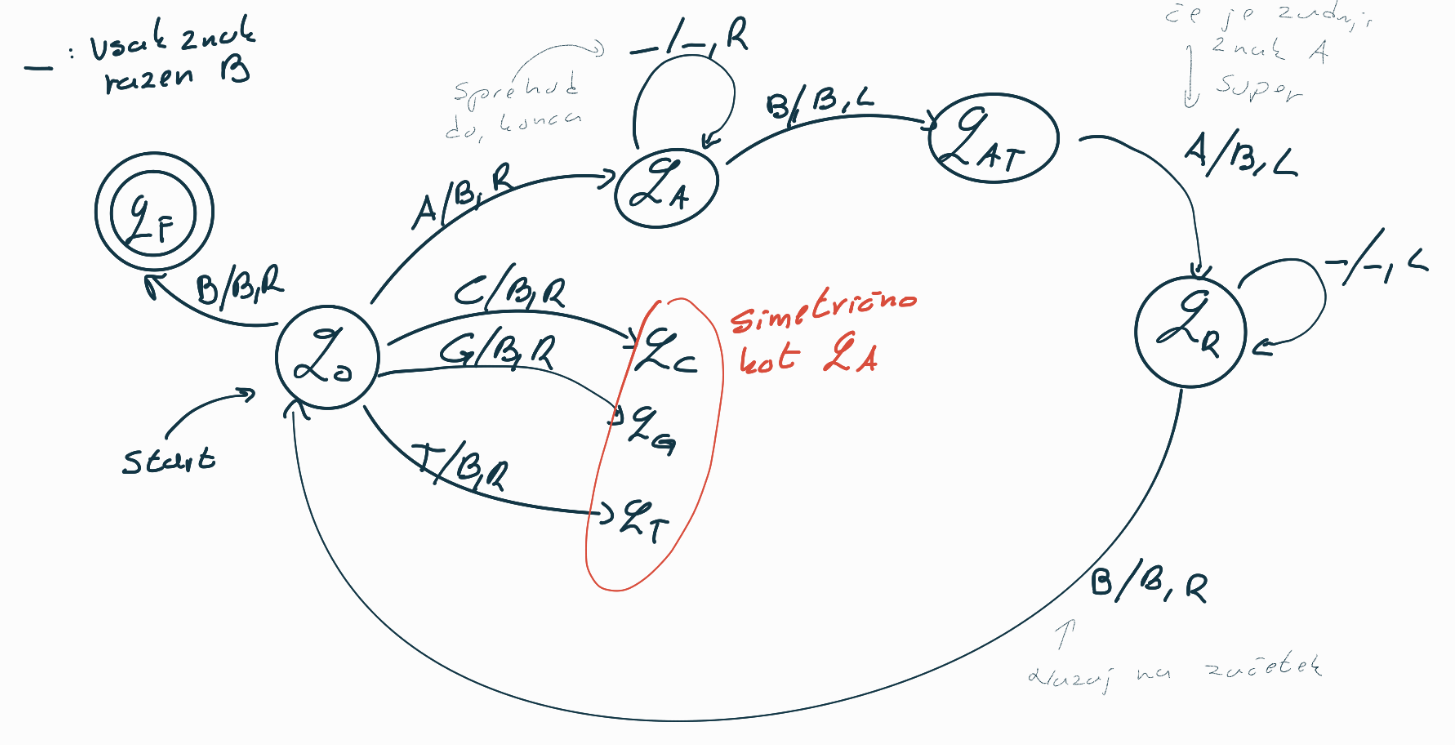
\includegraphics[width=\textwidth]{sedma.png}

\subsection{8. Naloga}
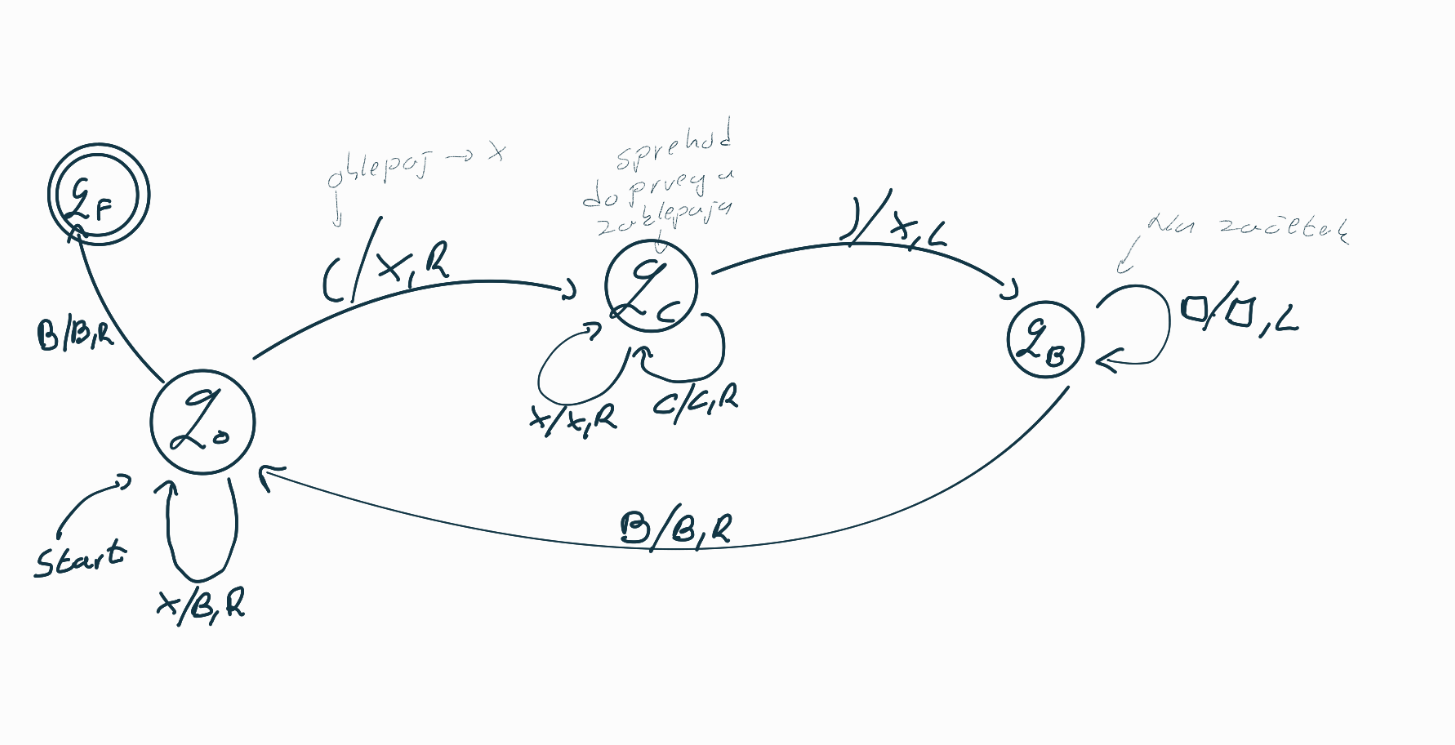
\includegraphics[width=\textwidth]{osma.png}

\subsection{9. Naloga}
Rešitev za to nalogo lahko najdete na povezavi: 

https://www.geeksforgeeks.org/construct-turing-machine-language-l-ww-w-01/

Tu bom priložil le sliko rešitve:
\n

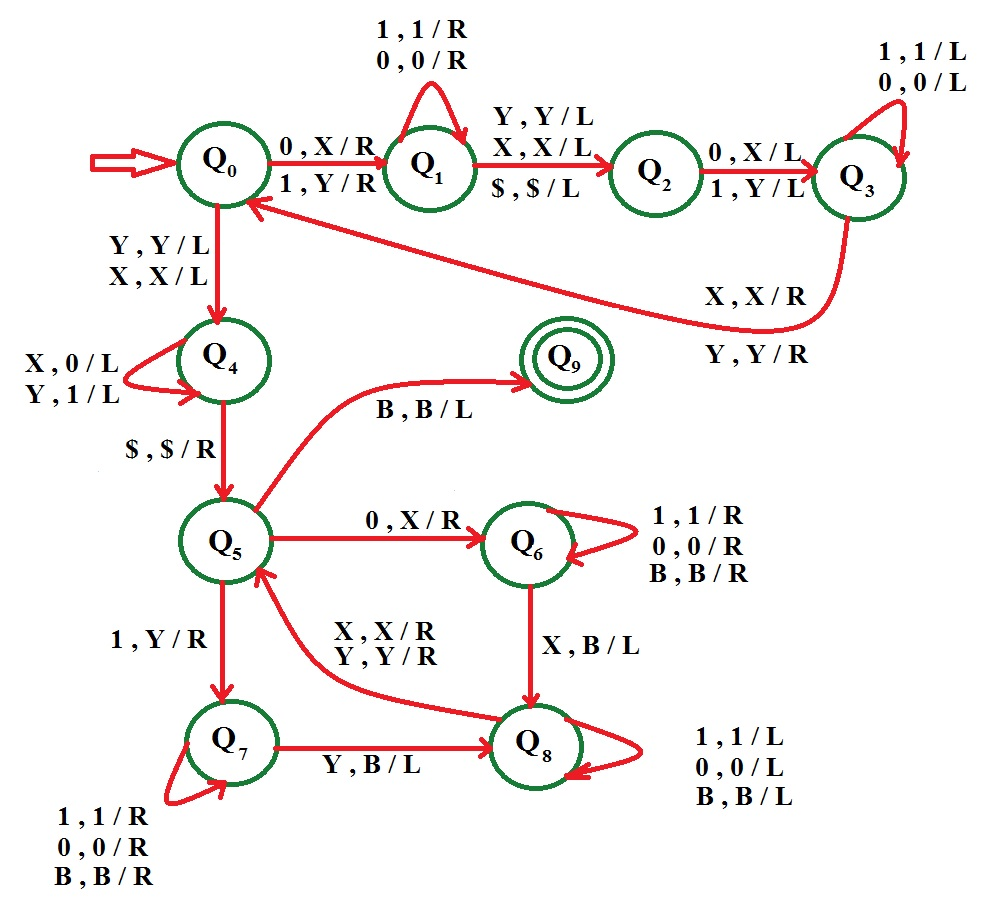
\includegraphics[width=\textwidth]{4-21.jpg}

\section{Drevesa}
\subsection{10. Naloga}
Resitev je v prilozeni datoteki.
\end{document}